\chapter*{Introduction}
\addcontentsline{toc}{chapter}{Introduction}

%% todo: ty protocols jsou rules a napojit to na ty ofnka
% Priklad predelat jen na JSON, to XML tam nedava smysl. Vzpomen si na priklad se SISem

During the software development process, we may come to a point where splitting a large monolithic codebase into smaller, well-defined modules is necessary to maintain the growth of our software. Using existing systems and connecting them is also a viable approach to building software. \cite{newman_monolith_nodate} In both cases, we end up with many applications and services that work as one.

This approach reduces complexity and demands on software developers as each part can be maintained, deployed, and tested separately. Each developer team must know only the portion they maintain and the immediate surrounding. The surrounding is then defined by a set of rules - an agreement specifying the data which flows between the systems.

Those rules must be created, documented, and kept up-to-date, which can be a long, error-prone task. The result of the process is usually a set of data schemas and documentation for developers. Especially the schemas need to be designed carefully to be, if possible, consistent in format and naming.

Data schemas are computer-readable documents that define the format of the data. They specify how data are structured and how individual properties are named with their possible values. The schemas are used to validate data produced by the application to ensure its correct format and can be used by humans to understand the expected format.

\medskip

As an example, consider a company selling and distributing its own goods. The goods are stored in warehouses and then shipped to customers. For the shipping process, the warehouse workers need to know the properties of the items they need to send. Similarly, customers need to know the properties of items they are buying. This scenario is denoted in \autoref{fig:company-schema}.

\begin{figure}[h]\centering
  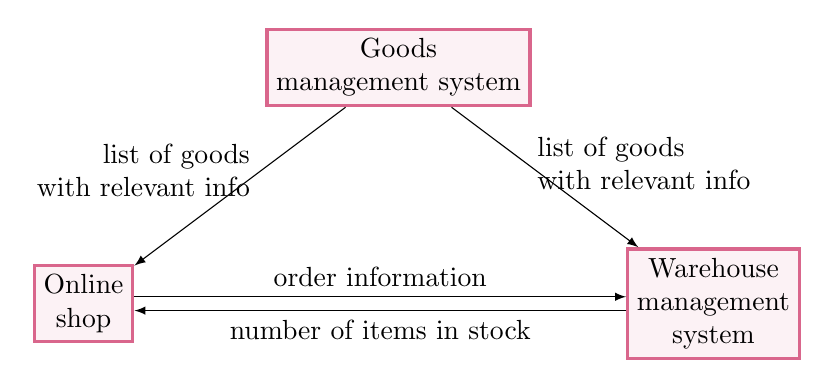
\begin{tikzpicture}[
    squarednode/.style={rectangle, draw=purple!60, fill=purple!5, very thick, minimum size=5mm,align=center},
]
    %Nodes
    \node[squarednode] (db) {Goods\\management system};
    \node[squarednode] (warehouse) at (4,-3) {Warehouse\\management\\system};
    \node[squarednode] (shop) at (-4,-3) {Online\\shop};

    %Lines
    \draw[-latex] (db) -- node[align=left,right=.5,pos=0.4]{list of goods\\with relevant info} (warehouse);
    \draw[-latex] (db) -- node[align=right,left=.5,pos=0.4]{list of goods\\with relevant info} (shop);
    \begin{scope}[transform canvas={yshift=.25em}]
        \draw[-latex] (shop) -- node[above,align=center]{order information} (warehouse);
    \end{scope}
    \begin{scope}[transform canvas={yshift=-.25em}]
        \draw[-latex] (warehouse) -- node[below,align=center]{number of items in stock} (shop);
    \end{scope}
  \end{tikzpicture}
  \caption{Example of the company architecture. The nodes are individual systems that communicate with each other.}
  \label{fig:company-schema}
\end{figure}

To describe the data that are being sent between the goods management system and both the online shop and the warehouse, we need to make two "agreements." Although both describe goods, the warehouse may require different properties than the shop. The \textit{name} and \textit{weight} of the items is essential for both systems, but the shop also requires the \textit{price}, contrary to warehouse that needs \textit{storing requirements}.

Furthermore, these properties are also reflected in the database schema design of the individual modules. The goods management has a database of goods, whether warehouse management only stores the position of individual goods in the warehouse and the information of warehouses, which are sent to the shop.

\medskip

Designing the schemas with supporting documentation by hand is a tedious task, and we may find several obstacles during the process, especially when the schema design is not made carefully:

\begin{enumerate}
    \item We need to describe the same thing for every schema that uses it. Hence doing the \textbf{same work multiple times}. \textit{From the example above, the name and weight of the item are used in two different schemas.}
    \item There is a high chance of \textbf{inconsistency}. We may name the semantically identical things differently, which may confuse software engineers who came in touch with multiple system parts. \textit{For example, the "name" of the item sold can be interchanged with "label" or "title" in another schema.}
    \item It is hard to introduce changes as we need to address all affected areas and modify them. If the change is made incrementally, we may lose the context of what is outdated and what is new.
\end{enumerate}

In addition to these obstacles, it is hard to provide supporting documentation, diagrams, and examples.

\bigskip

JSON is an example of a popular format that is widely used to exchange data between the server and the web page as it is natively supported by the web browser. To specify the structure, we can use JSON schema (see \autoref{fig:json-schema}), a document written in JSON format.

\begin{figure}[h]
\begin{verbatim}
{
  "$schema": "https://json-schema.org/draft/2020-12/schema",
  "title": "Item",
  "description": "Single item that can be sold in the store.",
  "type": "object",
  "required": [],
  "properties": {
    "name": {
      "type": "string",
      "title": "Item full name",
      "description": "Descriptive, short text, usually provided
                      by the manufacturer."
    },
    "price": {
      "type": "object",
      "title": "price",
      ...
    }
  }
}
\end{verbatim}
\caption{Example of JSON Schema that may describe the data being send between the Goods management system and the online shop.}
\label{fig:json-schema}
\end{figure}

\textbf{Diagrams} are images that visually explain the domain or data structure. \autoref{fig:json-schema} and \ref{figure:pim-example} can be considered as examples of diagrams that may help to better understand the structure. Diagrams are especially helpful in showing relations between different things that are used in schemas. For example, the order is made by a user, consisting of goods stored in warehouses.

\textbf{Examples} can be provided on two levels. Programmers may appreciate sample data that are valid against the schema and can be used to test their applications. \autoref{analysis:inheritance:json-data} is an example, although it would be better to provide more than two items. Examples can be provided for individual things as well. Someone may not be sure how long the ideal description is or what is the naming convention of items.

The \textbf{documentation} would describe each property of the schema in more detail in human-readable form. For example, documentation may be a website with multiple pages where the schema, diagrams, and examples are included, and all properties are described in formatted text. Individual things may be interlinked to ease the discovery of related things.

\bigskip

Future modifications to the system or changes in user requirements may enforce altering the schemas. Formally, the process of changing schemas is an \textbf{evolution}. The evolution is complex, as there can already be existing data that conform to the changed schemas. In that scenario, properly implementing a change in a user requirement requires modifying affected schemas, documentation, and all the data (in case the data are stored in the given format).

\begin{showcase}
    As an example, suppose that the address provided by a customer to deliver the goods is represented in multiple parts as \textit{street}, \textit{city}, \textit{zip code}, etc. We may decide that it would be better to have everything in one field as some parts of the address may be missing or not granular enough. The evolution in this case would mean to change all the schemas, documentation and examples to reflect the new structure, and possibly create transformation scripts to convert old data to the new format.
\end{showcase}

\section*{Ontology}
\addcontentsline{toc}{section}{Ontology}
%N Nerozumím, co tady znamená to "tends us". Jako že nás příklad vede k nějakému formálnímu popisu? Moc tomu nerozumím. Ale řekl bych spíš, že ten příklad naznačuje, že problém návrhu interfaců v komplexním systému (tj. systému, který má více než jeden interface) je potřeba vnímat na dvou rovinách - technická rovina definice datových struktur a jejich popisu a konceptuální / ontologická rovina nad tím, která zachycuje věcnou podstatu bez technických detailů. A že tato rovina se obvykle vyjadřuje v podobě ontologie.

The full process of designing schemas needs to be perceived on two levels. (i) On a technical level, where a user creates the schemas and describes the rules, (ii) and on a conceptual level, where the things and the relations between them are defined. The later level is called an \textbf{ontology}.

An ontology describes and names relations between the concepts from a real life without the technical details. Concepts are \textit{order}, \textit{customer}, or \textit{goods} in our case. Relations then specify, for example, that \textit{the order belongs to a customer} and \textit{consists of goods}.

Having an ontology properly defined is a step in the right direction as it gives us a template for schema modeling. All constructs that we may need to use are defined in the ontology, which ensures consistency across schemas and helps to avoid mistakes.

\medskip

With the data on the web \cite{data-on-the-web} trend in the last few years, even ontologies are becoming accessible publicly. Popular formats include RDFS (or RDF Schema) \footnote{\url{https://www.w3.org/TR/rdf-schema/}}, OWL\footnote{\url{https://www.w3.org/OWL/}}, UFO \cite{ufo22}, schema.org, and Wikidata\footnote{\url{https://www.wikidata.org/}}. For example, schema.org is a proprietary format describing useful data for search engines, such as events, organizations, or places.

Using pre-defined ontologies in a semi-automatic way of defining schemas is beneficiary because a schema designer may focus entirely on the schema structure and not on the domain semantics.

\section*{An alternative problem}
\addcontentsline{toc}{section}{An alternative problem}

In the section above, we have introduced a problem behind data modeling during software development as it is hard and time-consuming to design schemas properly. Nevertheless, schema design may be used in a wider environment to create recommendations for publishing various data in a unified format.

This task is usually undertaken by the state administration to ensure interoperability between various state and private organizations. The European Union enforces this in the directive 2019/1024 of the European Parliament, that data of public institutions shall be published as open data on the Internet in all formats it was created and, if possible, in a machine-readable format.

\medskip

\textbf{Open data} is a term for data published on the web without any restrictions on use. This means that anyone can use, modify and distribute the data for any reason, including commercial use.

The definition of open data is very loose but can be further specified by a 5-star scheme designed by Sir Tim Berners-Lee. Each star adds a restriction up until the fifth star describing the Linked Open Data.
\begin{itemize}[noitemsep,leftmargin=2cm]
    \item [1 $\bigstar$] Data are published on the web and can be used freely.
    \item [2 $\bigstar$] Data are structured and in a machine-readable format.
    \item [3 $\bigstar$] The format is not proprietary; hence anyone can open them.
    \item [4 $\bigstar$] Data uses RDF and SPARQL standards from W3C.
    \item [5 $\bigstar$] Data are linked to other data creating a network of data.
\end{itemize}

\medskip

The act then specifies \textbf{FOSes}\footnote{\url{https://eur-lex.europa.eu/legal-content/en/TXT/?uri=CELEX\%3A32019L1024}} \textit{(Formal Open Standard)} as recommendations for publishing selected categories of data, such as information about \textit{Tourist destinations} and \textit{Sports centers}. The purpose of these documents is to standardize how these data are published, usually by defining JSON and XML schemas along with textual documentation.

The process of designing those recommendations is comparable to designing schemas for a software system mentioned above - the designer needs to create schemas and documentation for them with examples and images.

Besides the different use cases, the process of designing the specification is slightly different, as we need to provide multiple formats, compared to the previous example, where a single format is sufficient. This brings us to several other challenges that are usually related to ease of the publications of the data:
\begin{enumerate}
  \item As there are multiple different formats, to not restrict the publishers, we need to design tools that can convert data between those formats. Because the conversion depends strictly on the schema, it is related directly to the schema modeling.
  \item To ensure the publishers that data are published correctly, we shall provide them with a platform for testing. This is also significantly related to schema modeling, as the purpose of the platform is to visualize the provided data to show that everything works.
\end{enumerate}

\section*{Focus of the work}
\addcontentsline{toc}{section}{Focus of the work}

This thesis analyzes and extends a newly created tool, Dataspecer \cite{dataspecer}, and formally defines and analyzes its internal framework, which follows the previous research \cite{necasky2007xsem, necasky2012conceptual} in the XML data modeling area and extends it to support new requirements.

The purpose of the tool is to ease the process of creation and management of data specifications, such as XSD, JSON Schema, and CSV Schema, and the creation of supplementary documents. The tool shall help users model schemas by providing relations from the chosen ontology and automatically performing manual work.

Supplementary documents are automatically generated files from the modeled schemas, such as the documentation, examples, diagrams, transformation scripts, and others.

\medskip

The tool is part of the larger ecosystem of tools, libraries, and frameworks for data modeling, which is being developed by the same authors.

Due to the complexity of the topic, this thesis does not attempt to cover and implement all features, as some of them will be kept for the authors' future work.

The purpose of this thesis is to provide basic formalisms and findings for the next work in this area.

\bigskip

The rest of the thesis is organized as follows. The following \autoref{chapters:related-work} analyzes related work and introduces the previous works as the common ground this work will follow - precisely the model-driven approach for data modeling and evolution of XML documents. The succeeding \autoref{chapters:analysis} analyzes new requirements for the tool and proposes a solution to some of them. The rest is only briefly analyzed to set a direction for future development. The next \autoref{chapters:implementation} identifies key implementation decisions and describes them. The last \autoref{chapters:evaluation} evaluates the tool in the context of use in modeling FOSes for the Czech Republic.

